\onehalfspacing
\section{Đề số 2}
\graphicspath{{./img/}}
\begin{bt} 
    \hfill
    \begin{enumerate}[a.]
        \item Thực hiện phép tính: $\mathrm{A}=\frac{2^{12} \cdot 3^5-4^6 \cdot 9^2}{2^2 \cdot 3^6+8^4 \cdot 3^5}-\frac{5^{10} .7^3-25^5 .49^2}{125.7^3+5^9 \cdot 14^3}$
        \item Tính giá trị biểu thức: $\quad B=1.2 .3+2.3 .4+3.4 .5+4.5 .6+\ldots+17.18 .19$
        \item Tìm một số tự nhiên có 3 chữ số, biết rằng nếu tăng chữ số hàng trăm thêm $\mathrm{n}$ đơn vị đồng thời giảm chữ số hàng chục và giảm chữ số hàng đơn vị đi n đơn vị thì được một số có 3 chữ số gấp n lần số có 3 chữ số ban đầu.
    \end{enumerate}
\loigiai{
    \begin{enumerate}
        \item Ta có:
        $$
        \begin{aligned}
        & \mathrm{A}=\frac{2^{12} \cdot 3^5-4^6 \cdot 9^2}{2^2 \cdot 3^6+8^4 \cdot 3^5}-\frac{5^{10} \cdot 7^3-25^5 \cdot 49^2}{125 \cdot 7^3+5^9 \cdot 14^3}=\frac{2^{12} \cdot 3^5-2^{12} \cdot 3^4}{2^{12} \cdot 3^6+2^{12} \cdot 3^5}-\frac{5^{10} \cdot 7^3-5^{10} \cdot 7^4}{5^9 \cdot 7^3+5^9 \cdot 2^3 \cdot 7^3} \\
        & \mathrm{~A}=\frac{2^{12} \cdot 3^4 3-1}{2^{12} \cdot 3^5 3+1}-\frac{5^{10} \cdot 7^3 1-7}{5^9 \cdot 7^3 1+2^3} \\
        & \mathrm{~A}=\frac{2}{3 \cdot 4}-\frac{5 \cdot(-6)}{9} \\
        & \mathrm{~A}=\frac{1}{6}-\frac{-10}{3}=\frac{7}{2}
        \end{aligned}
        $$
        \item $$
        \begin{aligned}
        & 4 B=1 \cdot 2 \cdot 3 \cdot 4+2 \cdot 3 \cdot 4 \cdot(5-1)+3 \cdot 4 \cdot 5 \cdot(6-2)+\ldots+17 \cdot 18 \cdot 19 \cdot(20-16) \\
        & 4 B=1 \cdot 2 \cdot 3 \cdot 4+2 \cdot 3 \cdot 4 \cdot 5-1 \cdot 2 \cdot 3 \cdot 4+3 \cdot 4 \cdot 5 \cdot 6-2 \cdot 3 \cdot 4 \cdot 5+17 \cdot 18 \cdot 19 \cdot 20-16 \cdot 17 \cdot 18 \cdot 19 \\
        & 4 B=17 \cdot 18 \cdot 19 \cdot 20 \\
        & B=17 \cdot 18 \cdot 19 \cdot 5=29070
        \end{aligned}
        $$
        \item Gọi số có 3 chữ số cần tìm là $\overline{\mathrm{abc}}$ $(\mathrm{a}, \mathrm{b}, \mathrm{c}$ là $\mathrm{STN}$ có 1 chữ số, $\mathrm{a} \neq 0)$.
        Theo bài ra ta có: $\overline{(\mathrm{a}+\mathrm{n})(\mathrm{b}-\mathrm{n})(\mathrm{c}-\mathrm{n})}=\mathrm{n} \cdot \overline{\mathrm{abc}}$
        $$
        \begin{aligned}
        & \Rightarrow 100(\mathrm{a}+\mathrm{n})+10(\mathrm{~b}-\mathrm{n})+(\mathrm{c}-\mathrm{n})=\mathrm{n}(100 \mathrm{a}+10 \mathrm{~b}+\mathrm{c}) \\
        & \Rightarrow 100 \mathrm{a}+100 \mathrm{n}+10 \mathrm{~b}-10 \mathrm{n}+\mathrm{c}-\mathrm{n}=100 \mathrm{an}+10 \mathrm{~b}+\mathrm{cn} \\
        & \Rightarrow 100(\mathrm{n}-1) \mathrm{a}+10(\mathrm{n}-1) \mathrm{b}+(\mathrm{n}-1) \mathrm{c}=89 \mathrm{n} \\
        & \Rightarrow 89 \mathrm{n} \vdots \mathrm{n}-1 \text { mà }(89 ; \mathrm{n}-1)=1 \text { nên } n \vdots \mathrm{n}-1
        \end{aligned}
        $$
        Tìm được $\mathrm{n}=2$ \\ 
        Số có 3 chữ số cần tìm là 178.
    \end{enumerate}
} 
\end{bt}

\begin{bt}
    \hfill
    \begin{enumerate}[a.]
        \item Tìm các số $x, y, z$ biết rằng: $\quad 3 x=4 y, 5 y=6 z$ và $x y z=30$.
        \item Tìm $x$ biết:
    $$
    \left|\mathrm{x}-\frac{1}{2}\right|+\frac{3}{4}=\left|-1,6+\frac{3}{5}\right|
    $$
    \end{enumerate}
\loigiai{
    \begin{enumerate}
        \item Ta có:
        $$
        \begin{aligned}
        & \Rightarrow \frac{\mathrm{x}}{4}=\frac{\mathrm{y}}{3} ; \frac{\mathrm{y}}{6}=\frac{\mathrm{z}}{5} \Rightarrow \frac{\mathrm{x}}{8}=\frac{\mathrm{y}}{6}=\frac{\mathrm{z}}{5}=\mathrm{k} \Rightarrow\left\{\begin{array}{l}
        \mathrm{x}=8 \mathrm{k} \\
        \mathrm{y}=6 \mathrm{k} \\
        \mathrm{z}=5 \mathrm{k}
        \end{array}\right. \\
        & \mathrm{xyz}=30 \Rightarrow 8 \mathrm{k} \cdot 6 \mathrm{k} \cdot 5 \mathrm{k}=30 \Rightarrow 240 \mathrm{k}^3=30 \Rightarrow \mathrm{k}=\frac{1}{2} \\
        & \Rightarrow x=4, y=3, \mathrm{z}=\frac{5}{2}
        \end{aligned}
        $$
        \item Ta có:
        $$
        \begin{aligned}
        & \left|\mathrm{x}-\frac{1}{2}\right|+\frac{3}{4}=\left|-1,6+\frac{3}{5}\right| \\
        \Rightarrow & \left|\mathrm{x}-\frac{1}{2}\right|+\frac{3}{4}=\left|-\frac{8}{5}+\frac{3}{5}\right| \\
        \Rightarrow & \left|\mathrm{x}-\frac{1}{2}\right|+\frac{3}{4}=1 \Rightarrow\left|\mathrm{x}-\frac{1}{2}\right|=\frac{1}{4} \Rightarrow\left[\begin{array}{l}
        \mathrm{x}=\frac{3}{4} \\
        \mathrm{x}=\frac{1}{4}
        \end{array}\right.
        \end{aligned}
        $$
    \end{enumerate}
} 
\end{bt}

\begin{bt}
    \hfill
    \begin{enumerate}[1.]
        \item Cho hàm số $\mathrm{y}=\mathrm{f}(\mathrm{x})=(\mathrm{m}-1) \mathrm{x}$
           \begin{enumerate}[a.]
            \item Tìm m biết: $f(2)-f(-1)=7$.
            \item Cho $m=5$. Tìm $x$ biết $f(3-2 x)=20$
           \end{enumerate}
        \item Cho các đơn thức $\mathrm{A}=-\frac{1}{2} \mathrm{x}^2 \mathrm{yz}^2, \mathrm{~B}=-\frac{3}{4} \mathrm{xy}^2 \mathrm{z}^2, \mathrm{C}=\mathrm{x}^3 \mathrm{y}$
        
        Chứng minh rằng các đơn thức $\mathrm{A}, \mathrm{B}, \mathrm{C}$ không thể cùng nhận giá trị âm.
    \end{enumerate}
\loigiai{
    \begin{enumerate}[1.]
        \item \begin{enumerate}
            \item $$
            \begin{aligned}
& \text{Vì } \mathrm{f}(2)-\mathrm{f}(-1)=7 \Rightarrow(\mathrm{m}-2) \cdot 2-(\mathrm{m}-1) \cdot(-1)=7 \\
& \Rightarrow 2 \mathrm{~m}-4+\mathrm{m}-1=7 \\
& \Rightarrow 3 \mathrm{~m}-5=7 \Rightarrow \mathrm{m}=4
\end{aligned}$$
\item Với $\mathrm{m}=5$ ta có hàm số $\mathrm{y}=\mathrm{f}(\mathrm{x})=4 \mathrm{x}$
$$
\begin{aligned}
& \text{Vì } f(3-2 x)=20 \Rightarrow 4(3-2 x)=20 \\
& \Rightarrow 12-8 x=20 \Rightarrow x=-1
\end{aligned}
$$
        \end{enumerate}

\item Giả sử cả 3 đơn thức $A, B, C$ cùng có giá trị âm
$\Rightarrow$ A.B.C có giá trị âm. \\
Mặt khác: A.B.C $=\left(-\frac{1}{2} x^2 y z^2\right) \cdot\left(-\frac{3}{4} x y^2 z^2\right) \cdot x^3 y=\frac{3}{8} x^6 y^4 z^4$
$$
\text { Vì } \frac{3}{8} \mathrm{x}^6 \mathrm{y}^4 \mathrm{z}^4 \geq 0 \quad \forall x, y \Rightarrow \text { A.B.C } \geq 0 \quad \forall x ; y
$$
Ta thấy (1) mâu thuẫn với (2) $\Rightarrow$ điều giả sử sai.
Vậy ba đơn thức $A=-\frac{1}{2} x^2 y z^2, B=-\frac{3}{4} x y^2 z^2, C=x^3 y$ không thể cùng có giá trị âm.
    \end{enumerate}
} 
\end{bt}

\begin{bt}
    Cho $\triangle \mathrm{ABC}$ nhọn có góc $\mathrm{A}$ bằng $60^{\circ}$. Phân giác $\mathrm{ABC}$ cắt $\mathrm{AC}$ tại $\mathrm{D}$, phân giác $\mathrm{ACB}$ cắt $A B$ tại E. BD cắt $C E$ tại I.
    \begin{enumerate}[a.]
    \item Tính số đo góc BIC.
    \item Trên cạnh $\mathrm{BC}$ lấy điểm $\mathrm{F}$ sao cho $\mathrm{BF}=\mathrm{BE}$. Chứng minh $\Delta \mathrm{CID}=\Delta \mathrm{CIF}$.
    \item Trên tia IF lấy điểm $\mathrm{M}$ sao cho $\mathrm{IM}=\mathrm{IB}+\mathrm{IC}$. Chứng minh $\triangle \mathrm{BCM}$ là tam giác đều.
    \end{enumerate}
\loigiai{
    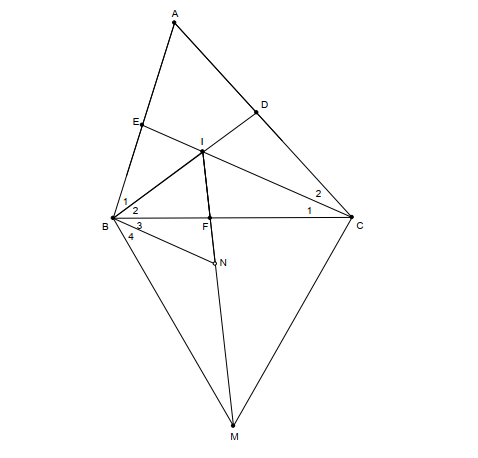
\includegraphics[width=0.7\textwidth]{2-4-lg.png}
    \begin{enumerate}
        \item $\mathrm{BD}$ là phân giác của góc $\mathrm{ABC}$ nên $\mathrm{B}_1=\mathrm{B}_2=\frac{1}{2} \mathrm{ABC}$
        $C E$ là phân giác của góc $A C B$ nên $C_1=C_2=\frac{1}{2} A C B$
        Mà tam giác $\mathrm{ABC}$ có $\mathrm{A}+\mathrm{B}+\mathrm{C}=180^{\circ}$ suy ra $60^{\circ}+\mathrm{ABC}+\mathrm{ACB}=180^{\circ}$
        $$
        \Rightarrow \mathrm{ABC}+\mathrm{ACB}=120^{\circ} \Rightarrow \mathrm{B}_2+\mathrm{C}_1=60^{\circ} \Rightarrow \mathrm{BIC}=120^{\circ}
        $$
        \item $\Delta \mathrm{BIE}=\Delta \mathrm{BIF}(\mathrm{cgc}) \Rightarrow \mathrm{BIE}=\mathrm{BIF}$
        $\mathrm{BIC}=120^{\circ} \Rightarrow \mathrm{BIE}=60^{\circ} \Rightarrow \mathrm{BIE}=\mathrm{BIF}=60^{\circ}$
        $\mathrm{Mà} \mathrm{BIE}+\mathrm{BIF}+\mathrm{CIF}=180^{\circ} \Rightarrow \mathrm{CIF}=60^{\circ}$
        $\mathrm{CID}=\mathrm{BIE}=60^{\circ}$ (đ.đ) $\Rightarrow \mathrm{CIF}=\mathrm{CID}=60^{\circ}$
        $\Rightarrow \Delta \mathrm{CID}=\Delta \mathrm{CIF}$ (g.c.g)
        \item Trên đoạn IM lấy điểm $\mathrm{N}$ sao cho $\mathrm{IB}=\mathrm{IN} \Rightarrow \mathrm{NM}=\mathrm{IC}$
        $\Rightarrow \Delta \mathrm{BIN}$ đều $\Rightarrow \mathrm{BN}=\mathrm{BI}$ và $\mathrm{BNM}=120^{\circ}$
        $\Rightarrow \Delta \mathrm{BNM}=\Delta \mathrm{BIC}$ (c.g.c)
        $\Rightarrow B M=B C$ và $B_2=B_4 \Rightarrow \Delta B C M$ đều
    \end{enumerate}
}
\end{bt}

\begin{bt}
    Tìm số tự nhiên $\mathrm{n}$ thỏa mãn điều kiện: $\quad 2 \cdot 2^2+3 \cdot 2^3+4 \cdot 2^4+\ldots+\mathrm{n} \cdot 2^{\mathrm{n}}=2^{\mathrm{n}+11}$
\loigiai{
    Đặt $S=2.2^2+3.2^3+4.2^4+\ldots+n .2^{\mathrm{n}}$
$$
\begin{aligned}
& S=2 S-S=\left(2 \cdot 2^3+3 \cdot 2^4+4 \cdot 2^5+\ldots+n \cdot 2^{n+1}\right)-\left(2 \cdot 2^2+3 \cdot 2^3+4 \cdot 2^4+\ldots+n \cdot 2^n\right) \\
& S=n \cdot 2^{n+1}-2^3-\left(2^3+2^4+\ldots+2^{n-1}+2^n\right)
\end{aligned}
$$
Đặt $\mathrm{T}=2^3+2^4+\ldots+2^{\mathrm{n}-1}+2^{\mathrm{n}}$. Tính được $\mathrm{T}=2 \mathrm{~T}-\mathrm{T}=2^{\mathrm{n}-1}-2^3$\\
$
\Rightarrow \mathrm{S}=\mathrm{n} \cdot 2^{\mathrm{n}+1}-2^3-2^{\mathrm{n}-1}+2^3=(\mathrm{n}-1) \cdot 2^{\mathrm{n}+1}
$
$\\
\Rightarrow(\mathrm{n}-1) \cdot 2^{\mathrm{n}+1}=2^{\mathrm{n}+11} \Rightarrow \mathrm{n}-1=2^{10} \Rightarrow \mathrm{n}=2^{10}+1=1025
$
}
\end{bt}